\section{Trees}
{\tiny a hierarchical, non-linear data structure \\
a graph with certain properties\\
in cl: parse trees, language trees, decision trees}\\
\scriptsize{Definitions}\\ {\tiny a set of nodes organized hierarchically with the following properties: \\
If a tree is non-empty, it has a special node root\\
Except the root node, every node in the tree has a unique parent (all nodes except the root are children of another node)\\
Alternatively, recursive definition:\\
the empty set of nodes is a tree\\
otherwise a tree contains a root with sub-trees as its children}\\
\scriptsize{siblings} {\tiny nodes with the same parent
}\\
\scriptsize{internal nodes} {\tiny nodes with children
}\\
\scriptsize{leaf nodes} {\tiny nodes without children
}\\
\scriptsize{path} {\tiny sequence of connected nodes
}\\
\scriptsize{ancestors/decendants} {\tiny any node in the path from the root to a particular node; a node is the descendant of its ancestors
}\\
\scriptsize{internal nodes} {\tiny nodes with children
}\\
\scriptsize{subtree} {\tiny a tree rooted by a non-root node
}\\
\scriptsize{depth} {\tiny number of edges from root
}\\
\scriptsize{height} {\tiny number of edges from the deepest descendant; the height of a tree is the height of its root
}\\
\scriptsize{Ordered trees}\\ 
{\tiny if there is an odering between siblings, e.g. document (e.g. HTML) structure tree, parse trees, family tree\\
in many cases order is not important (e.g. class hierarchy in object-oriented program, file tree in computer)
}\\
\scriptsize{Binary trees}\\
{\tiny nodes can have at most 2 children\\
have a natural order: left/right child\\
proper/full: if every node has either 2 children or none\\
complete: if every level except possibly the last is completely filled, all nodes at the last level is at the left\\
perfect: a full binary tree whose leaf nodes have the same depth\\
properties: for a binary tree with nl leaf nodes, ni internal nodes, n nodes and height h:\\
h+1 <= n <= 2**(h+1)-1\\
1 <= nl <= 2**h\\
h <= ni <= 2**h -1\\
log(n+1)-1 <= h <= n-1\\
for any proper binary tree: nl=ni+1
}\\
\scriptsize{Implementation} \\
{\tiny general case: linked data structure\\
arrays: root stored at index 0, left child of the node at index i stored at 2i+1, right child at 2i+2, parent at (i-1)/2 (if the binary tree is complete, this representation does not waste (much) space
}\\
\scriptsize{Breadth first traversal (level order)}\\ 
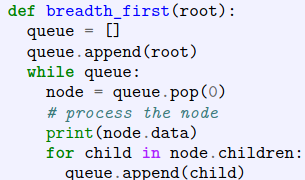
\includegraphics[scale=0.25]{breath_first.png}\\
\scriptsize{Pre-order traversal} \\
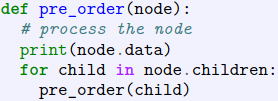
\includegraphics[scale=0.25]{pre-order.png}\\
\scriptsize{Post-order traversal} \\
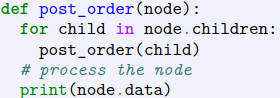
\includegraphics[scale=0.25]{post-order.png}\\
\scriptsize{In-order traversal} \\
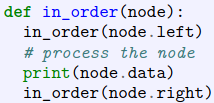
\includegraphics[scale=0.25]{in-order.png}